\documentclass[11pt]{article}
\usepackage[margin=1in]{geometry}
\usepackage[T1]{fontenc}
\usepackage[utf8]{inputenc}
\usepackage{amsmath,amssymb,amsthm}
\usepackage{graphicx}
\usepackage{float}
\usepackage{xcolor}
\usepackage{microtype}
\usepackage[colorlinks=true,linkcolor=blue!55!black,citecolor=blue!55!black,urlcolor=blue!55!black]{hyperref}

\newtheorem{theorem}{Theorem}
\newtheorem{corollary}{Corollary}
\newcommand{\C}{\mathbb C}
\newcommand{\R}{\mathbb R}

\title{Exact classification of rank-one orthogonal projections that are $\ell^\infty$-contractive}
\author{Candidate full-solution packet for arXiv:0903.3580}
\date{11 August 2026}

\begin{document}
\maketitle

\begin{center}
\fbox{\parbox{0.92\textwidth}{\textbf{Status: candidate full solution, likely valid, subject to human review.}
For a unit vector $v\in\C^N$, the orthogonal projection $P_v=vv^*$ is
$\ell^\infty$-contractive if and only if all nonzero coordinates of $v$ have
the same modulus.  Applying this dimension-free criterion to the spherical
coordinates in arXiv:0903.3580 gives an exact parameter list and proves that
no pairs beyond the families already observed in the source exist.}}
\end{center}

\section{Source question}

Mugnolo studies heat semigroups on a three-edge star with one-dimensional
boundary space $Y_{\xi,\phi}\subset\C^3$.  In the real spherical chart, this
space is generated by
\begin{equation}\label{eq:v}
 v_{\xi,\phi}=(\sin\xi\cos\phi,\ \sin\xi\sin\phi,\ \cos\xi),
 \qquad \xi,\phi\in[0,\pi),
\end{equation}
and its orthogonal projection is $P_{Y_{\xi,\phi}}=v_{\xi,\phi}
v_{\xi,\phi}^{\mathsf T}$.  The source reduces $L^\infty$-contractivity of
the associated heat semigroup (with $S=0$) to $\ell^\infty$-contractivity of
this matrix, plots the three absolute row sums, and verifies several isolated
points and decoupled families.  It then states \cite[p.~19]{source}:
\begin{quote}
``We do not know whether further pairs $(\xi,\phi)$ leading to
$L^\infty$-contractivity exist.''
\end{quote}
The relevant source pages are reproduced in Appendix~\ref{app:evidence}.

\section*{Idea of the proof}

There is no need to solve three trigonometric inequalities.  The absolute row
sum of the rank-one matrix $vv^*$ is $|v_i|\sum_j|v_j|$, so its largest row
sum is $\lVert v\rVert_\infty\lVert v\rVert_1$.  If $v$ is a unit vector and
$m=\lVert v\rVert_\infty$, then
\[
 1=\sum_i|v_i|^2\le m\sum_i|v_i|.
\]
Contractivity forces equality.  Its defect is the sum of the nonnegative
terms $|v_i|(m-|v_i|)$, so equality occurs exactly when each coordinate has
modulus either zero or $m$.  The spherical parameter list then follows by
separating supports of sizes one, two, and three.

\section{A dimension-free classification}

\begin{theorem}\label{thm:general}
Let $v=(v_1,\ldots,v_N)\in\C^N$ satisfy $\lVert v\rVert_2=1$, and let
$P_vx=\langle x,v\rangle v$ be the orthogonal projection onto $\C v$.
Then
\begin{equation}\label{eq:norm}
 \lVert P_v\rVert_{\ell^\infty_N\to\ell^\infty_N}
 =\lVert v\rVert_\infty\lVert v\rVert_1\ge1.
\end{equation}
Moreover, the following are equivalent:
\begin{enumerate}
\item $P_v$ is $\ell^\infty$-contractive;
\item every nonzero coordinate of $v$ has the same modulus;
\item for some nonempty support $S\subset\{1,\ldots,N\}$,
\[
 |v_i|=|S|^{-1/2}\quad(i\in S),
 \qquad v_i=0\quad(i\notin S).
\]
\end{enumerate}
\end{theorem}

\begin{proof}
The $(i,j)$ entry of $P_v=vv^*$ has modulus $|v_i||v_j|$.  The induced
$\ell^\infty$ norm is the largest absolute row sum, hence
\[
 \lVert P_v\rVert_{\infty\to\infty}
 =\max_i\sum_j|v_i||v_j|
 =\lVert v\rVert_\infty\lVert v\rVert_1.
\]
Put $m=\lVert v\rVert_\infty$.  Since $|v_i|\le m$,
\begin{equation}\label{eq:defect}
 1=\sum_i|v_i|^2\le m\sum_i|v_i|
 =\lVert P_v\rVert_{\infty\to\infty}.
\end{equation}
Thus contractivity is equivalent to equality in \eqref{eq:defect}.  But the
defect is
\[
 m\sum_i|v_i|-\sum_i|v_i|^2
 =\sum_i |v_i|(m-|v_i|),
\]
a sum of nonnegative numbers.  It vanishes exactly when
$|v_i|\in\{0,m\}$ for every $i$.  If the nonzero support has size $k$, unit
normalization gives $km^2=1$, hence $m=k^{-1/2}$.  The converse is immediate.
\end{proof}

The theorem also permits arbitrary complex phases on the nonzero coordinates.
For the source's real spherical family, only signs occur.

\section{Complete answer in the source coordinates}

Let
\[
 \alpha:=\arctan\sqrt2\in(0,\pi/2).
\]

\begin{corollary}\label{cor:list}
For $(\xi,\phi)\in[0,\pi)^2$, the projection
$P_{Y_{\xi,\phi}}$ in the source is $\ell^\infty$-contractive if and only if
$(\xi,\phi)$ belongs to
\begin{align}\label{eq:list}
 &\bigl(\{0\}\times[0,\pi)\bigr) \\
 &\quad{}\cup
 \left(\left\{\frac\pi2\right\}\times
 \left\{0,\frac\pi4,\frac\pi2,\frac{3\pi}4\right\}\right) \\
 &\quad{}\cup
 \left(\left\{\frac\pi4,\frac{3\pi}4\right\}\times
 \left\{0,\frac\pi2\right\}\right) \\
 &\quad{}\cup
 \left(\{\alpha,\pi-\alpha\}\times
 \left\{\frac\pi4,\frac{3\pi}4\right\}\right).
\end{align}
Consequently there are no further pairs in the chart considered by the
source.  With $S=0$, this is also the exact list of the corresponding
$L^\infty$-contractive heat semigroups, for both the time-independent and
dynamic boundary problems covered by the source's equivalence theorem.
\end{corollary}

\begin{proof}
Apply Theorem~\ref{thm:general} to \eqref{eq:v} and separate by support size.

If exactly one coordinate is nonzero, one obtains $\xi=0$ with arbitrary
$\phi$, or
\[
 (\xi,\phi)=(\pi/2,0)\quad\text{or}\quad(\pi/2,\pi/2).
\]

If exactly two coordinates are nonzero and have equal absolute value, the
support $\{1,2\}$ gives
\[
 \xi=\frac\pi2,\qquad
 \phi\in\left\{\frac\pi4,\frac{3\pi}4\right\};
\]
the support $\{1,3\}$ gives
\[
 \phi=0,\qquad
 \xi\in\left\{\frac\pi4,\frac{3\pi}4\right\};
\]
and the support $\{2,3\}$ gives
\[
 \phi=\frac\pi2,\qquad
 \xi\in\left\{\frac\pi4,\frac{3\pi}4\right\}.
\]

If all three coordinates are nonzero with equal absolute value, then
$|\cos\phi|=|\sin\phi|$, so
$\phi\in\{\pi/4,3\pi/4\}$.  Equality with the third coordinate then becomes
\[
 |\sin\xi|/\sqrt2=|\cos\xi|,
\]
or $|\tan\xi|=\sqrt2$.  Hence
$\xi\in\{\alpha,\pi-\alpha\}$.  Collecting the cases gives exactly
\eqref{eq:list}.
\end{proof}

Modulo the coordinate degeneracy at $\xi=0$, list~\eqref{eq:list} represents
thirteen real lines: three coordinate axes, six equal-modulus two-coordinate
lines, and four equal-modulus three-coordinate lines.  The source had already
exhibited these families; Corollary~\ref{cor:list} supplies the missing
exhaustiveness proof.

\section{Verification, scope, and novelty}

The argument is algebraic and exact.  The companion script
\texttt{code/verify\_classification.py} checks the norm formula on random
vectors, verifies all displayed parameter representatives, and confirms that
small perturbations of every nondegenerate solution have norm greater than
one.  These computations are sanity checks, not part of the proof.

This fully answers the printed question for one-dimensional boundary spaces
of $\C^3$ and strengthens it to rank-one orthogonal projections in every
finite dimension.  It does not classify higher-rank orthogonal projections,
nor does it settle the distinct question in the source about the complements
$I-P_{Y_{\xi,\phi}}$.

The bounded novelty check on 11 August 2026 searched the run registry and its
solution, attempt, and proof-gap indexes for the arXiv id, title, and central
projection/contractivity phrases.  Exact-title, exact-question, and
rank-one-projection primary-source web searches found the source paper and
general literature on contractive projections, but no later paper giving this
parameter classification or answering the quoted question.  Because the
argument is elementary, this is not an exhaustive priority claim.

\textbf{Human-review recommendation.} Check that the source's reduction from
semigroup contractivity to $\ell^\infty$-contractivity of
$P_{Y_{\xi,\phi}}$ is being used with $S=0$, as in its example section.  The
finite-dimensional classification itself is independent of the PDE setup.

\clearpage
\appendix
\section{Source-page evidence}\label{app:evidence}

\begin{figure}[H]
\centering
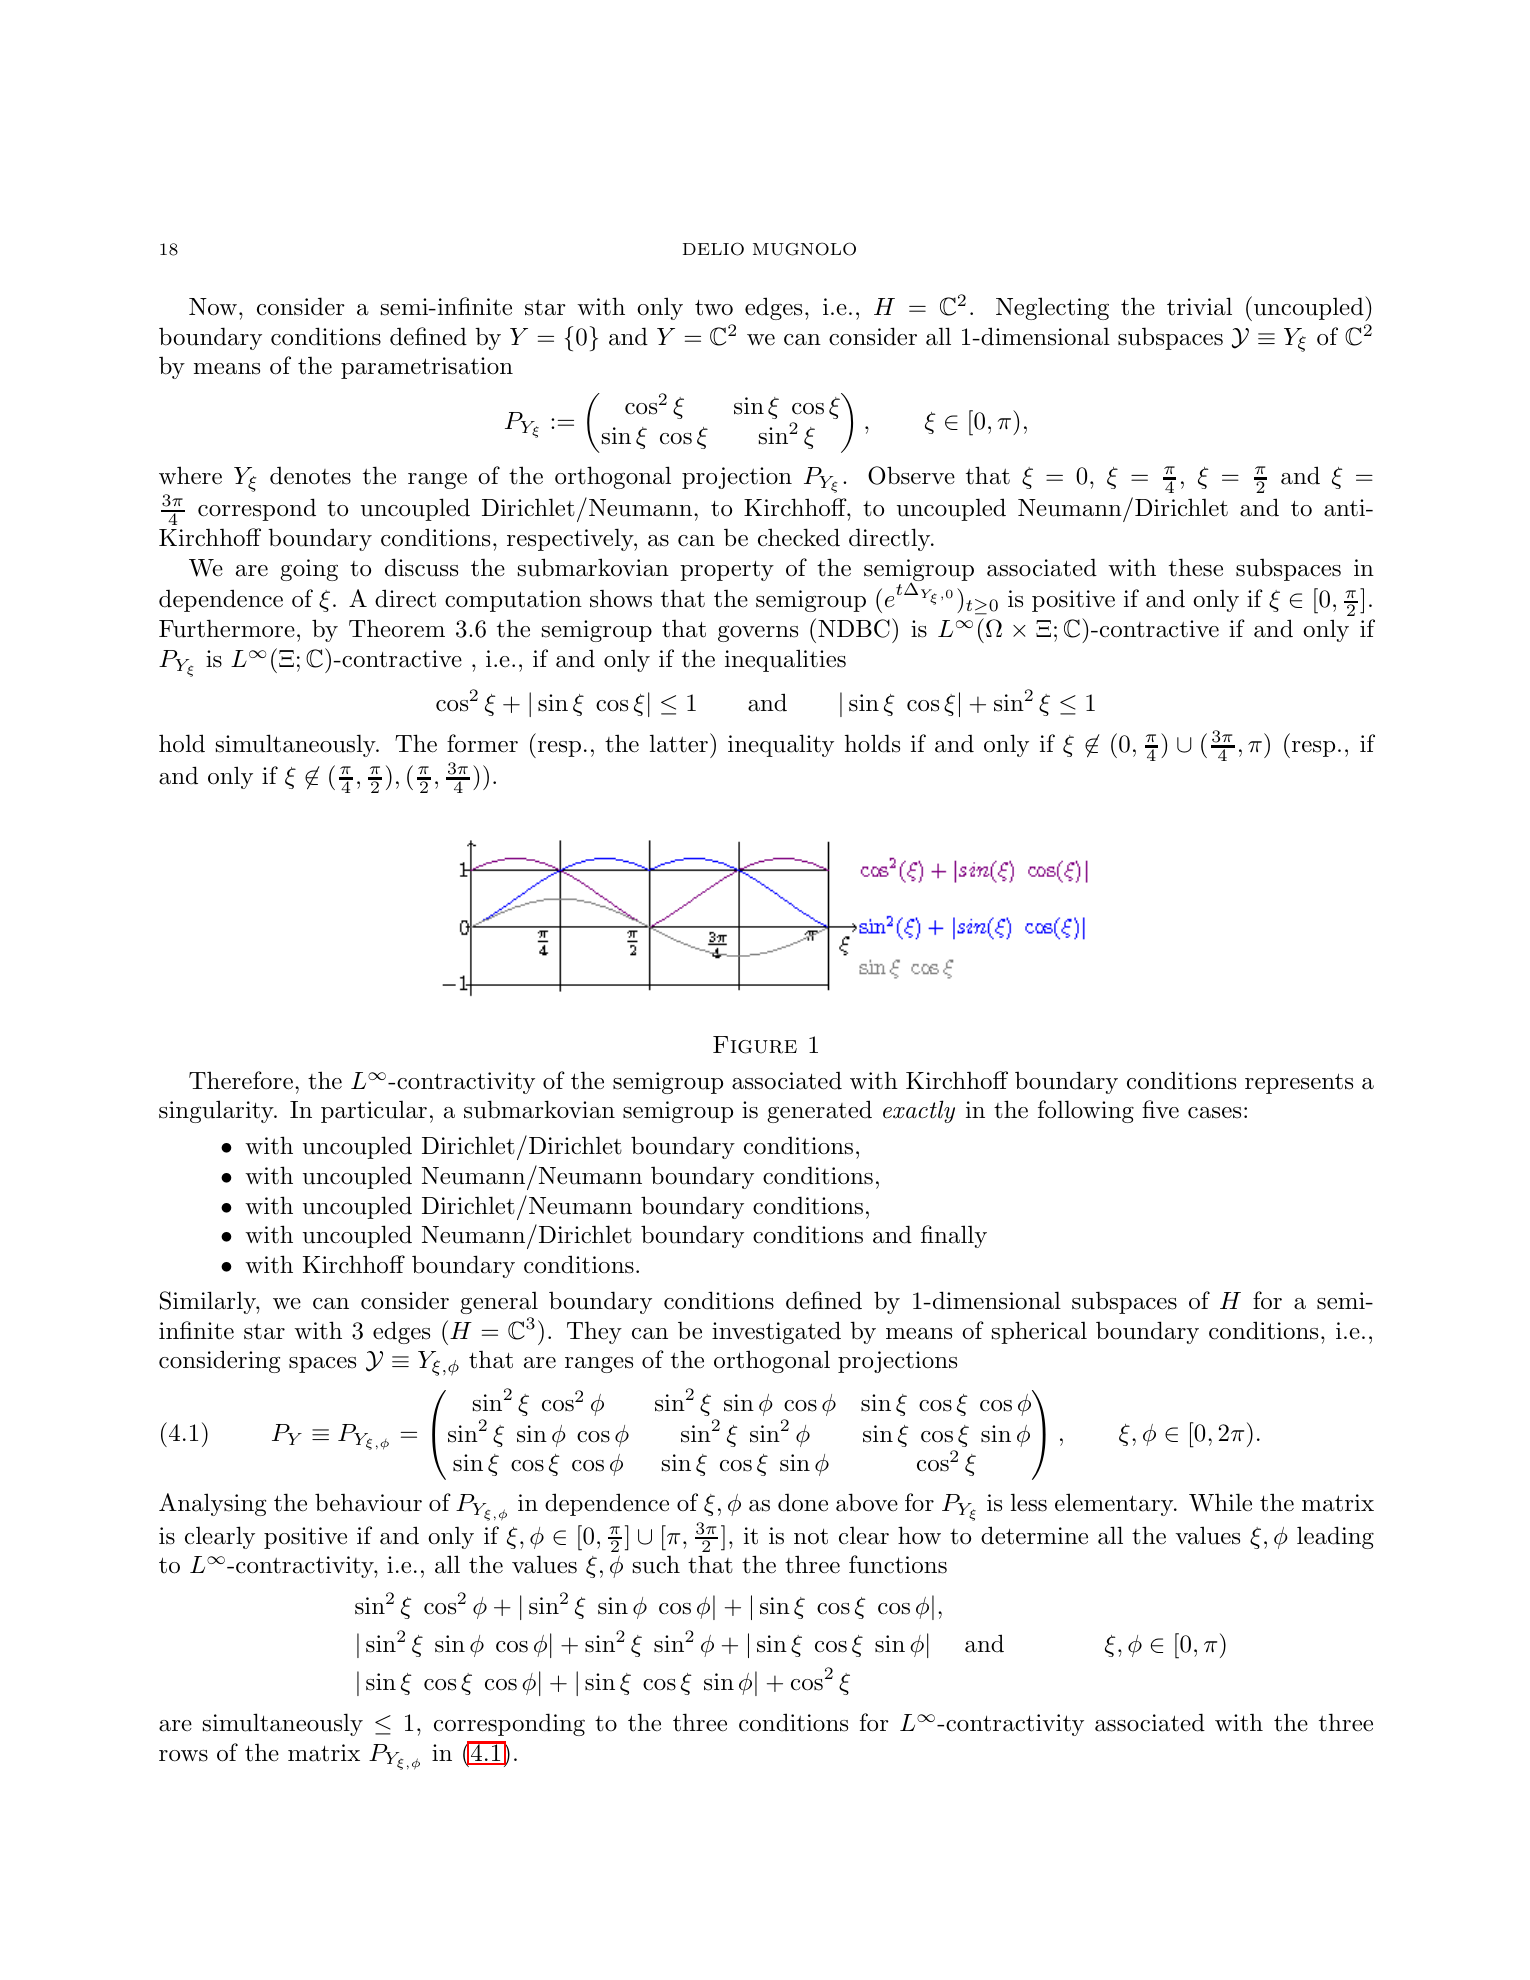
\includegraphics[height=0.70\textheight,keepaspectratio]{figures/source_setup.png}
\caption{Printed page 18 of arXiv:0903.3580, introducing the spherical
projection and reducing the question to three absolute row-sum inequalities.}
\end{figure}

\clearpage
\begin{figure}[H]
\centering

\includegraphics[height=0.70\textheight,keepaspectratio]{figures/source_question.png}
\caption{Printed page 19 of arXiv:0903.3580, listing the observed solutions
and asking whether further $L^\infty$-contractive parameter pairs exist.}
\end{figure}

\begin{thebibliography}{1}
\bibitem{source}
Delio Mugnolo,
\emph{Vector-valued heat equations and networks with coupled dynamic boundary
conditions}, arXiv:0903.3580, 2009.
\end{thebibliography}

\end{document}
